
\section{Measuring Time} \label{MeasuringTimeSection}

Although the measuring time is canceled in the antiproton to proton flux ratio calculation, it has to be determined due to the rigidity cutoff in the cuts and selections, which explains the low statistics in the low rigidity analysis. Also, in the time-dependent analysis, the measuring time in six Bartels Rotations helps to understand the antiproton number changes. Furthermore, in the MC simulation the rigidity cutoff is not simulated, this effect has to be corrected in unfolding. \par 

%% Definition: Measuring Time
The measuring time is the total time that all the sub-detectors are in nominal operation and could record events. Due to the detector's operation cuts and the trigger dead time, which is the time needed for readout, the measuring time is lower than the exposure time, which is the total data-taking time since the start of the experiment.   \par


%% LiveTime Fraction And Trigger 

\begin{figure}[htpb]
\centering
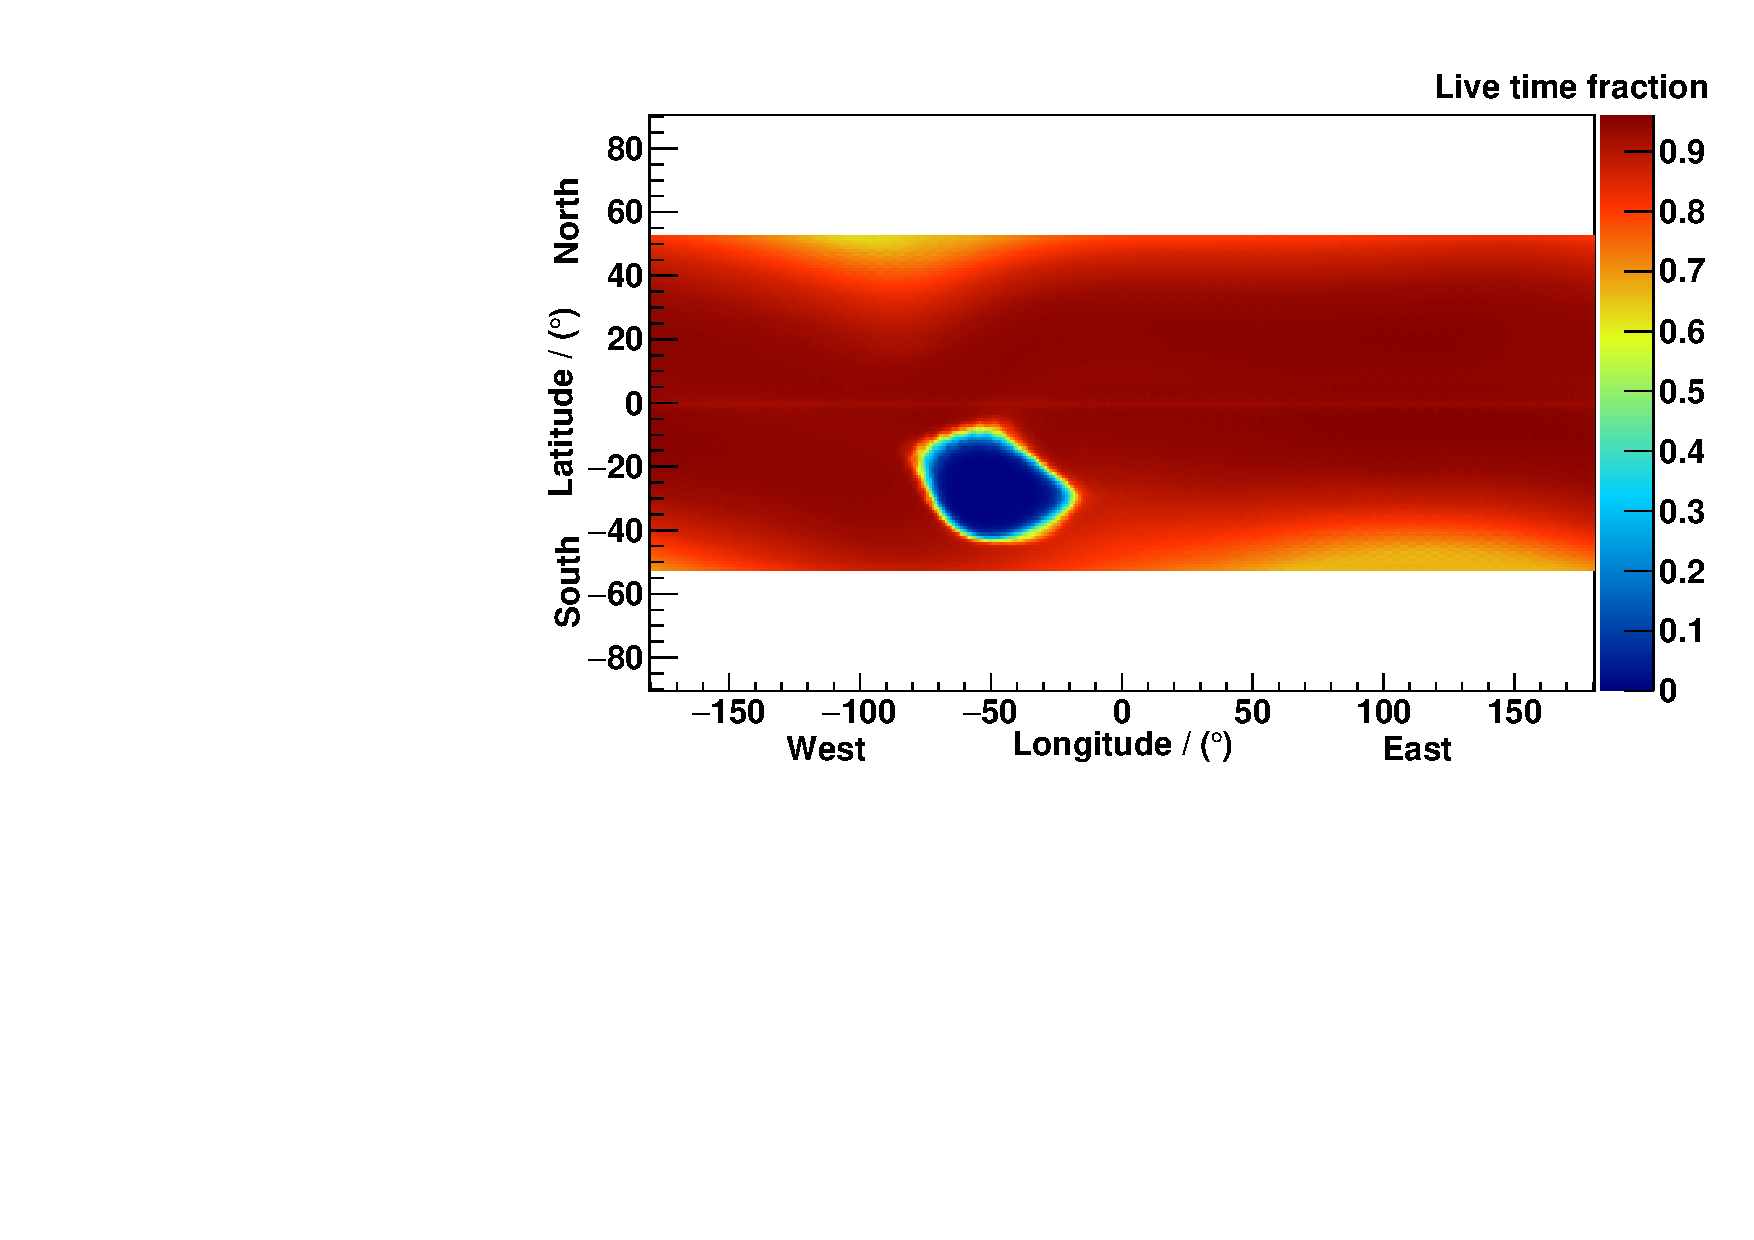
\includegraphics[width=1.0\textwidth]{Figures/chapter4/MeasuringTime/LiveTimeFractionVsISSPosition.pdf}
\caption[Live time fraction vs. ISS position.]{Live time fraction vs. ISS position. The live time fraction in the most areas is above 0.9 while in the SAA is extremely low due to plenty of low energy particles.}
\label{LiveTimeFractionVsISSPosition}
\end{figure}

Because of the trigger dead time, if the event trigger rate goes up and surpasses the threshold, then not all the events can be detected and recorded. Therefore, the live time fraction can be defined as the fraction of a second that the trigger is ready to record. Because the amount of incoming particles depends on the ISS position in the geomagnetic field, the live time fraction is close to one in most areas but less than one in high latitude areas, see figure \ref{LiveTimeFractionVsISSPosition}. Also, in the SAA, there are plenty of low energy particles going through the detector. Therefore, the trigger rate in this area is very high, and the live time fraction is very low correspondently. In figure \ref{MeasuringTimeVsLiveTime}, the measuring time as function of live time fraction is given. For the entire data-taking period, the live time fraction is mostly above 90\%.  \par
%In figure \ref{ParticlesVsTriggers}, the trigger vs. particles per trigger is presented.  \par
% In figure \ref{TriggerRateVsPosition}, the trigger rate vs ISS position is shown. 

% Start Comment out
%\begin{comment}
%\begin{figure}[]
%    \centering
%    \subfigure[]{
%        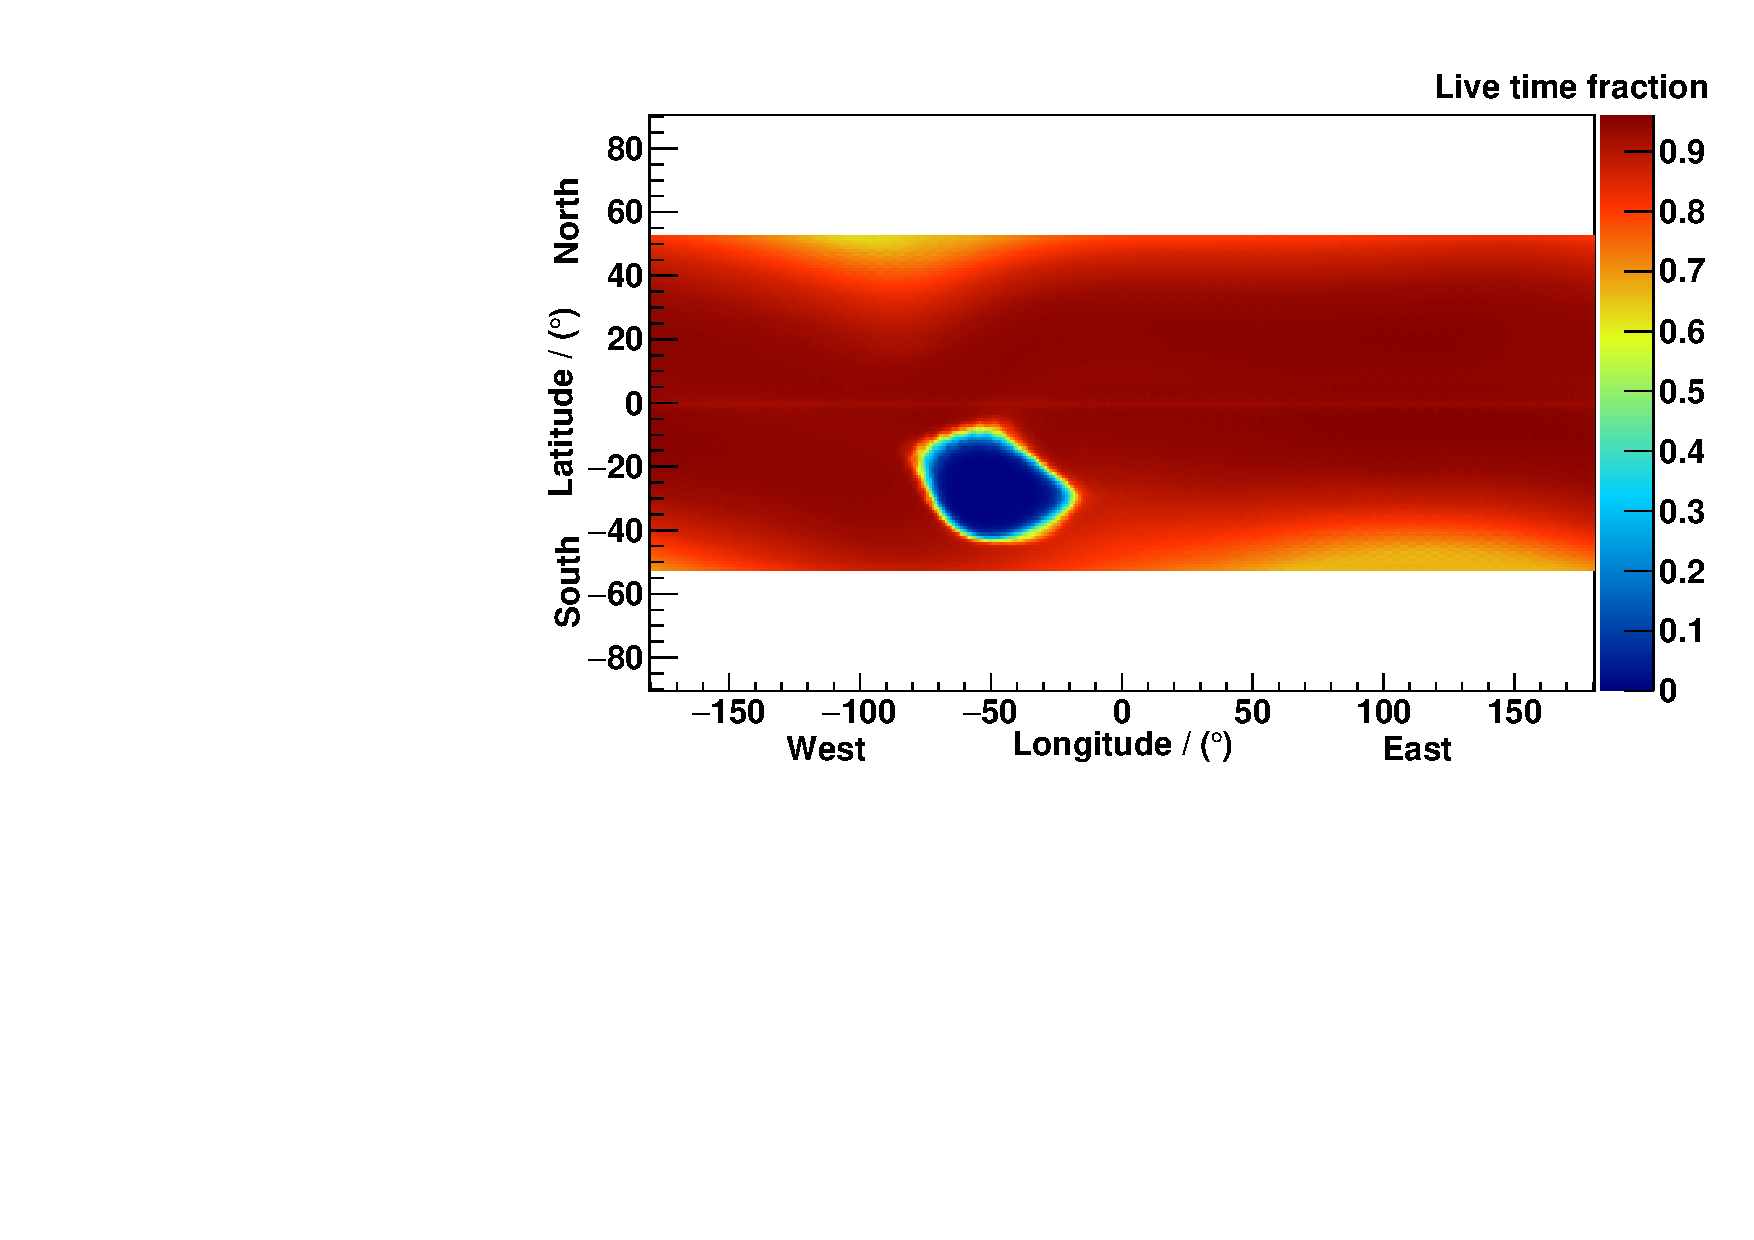
\includegraphics[width=0.47\textwidth, height=0.29\textheight]{Figures/chapter4/MeasuringTime/LiveTimeFractionVsISSPosition.pdf} 
%        \label{LiveTimeFractionVsISSPosition}
%    }
%    \subfigure[]{
%	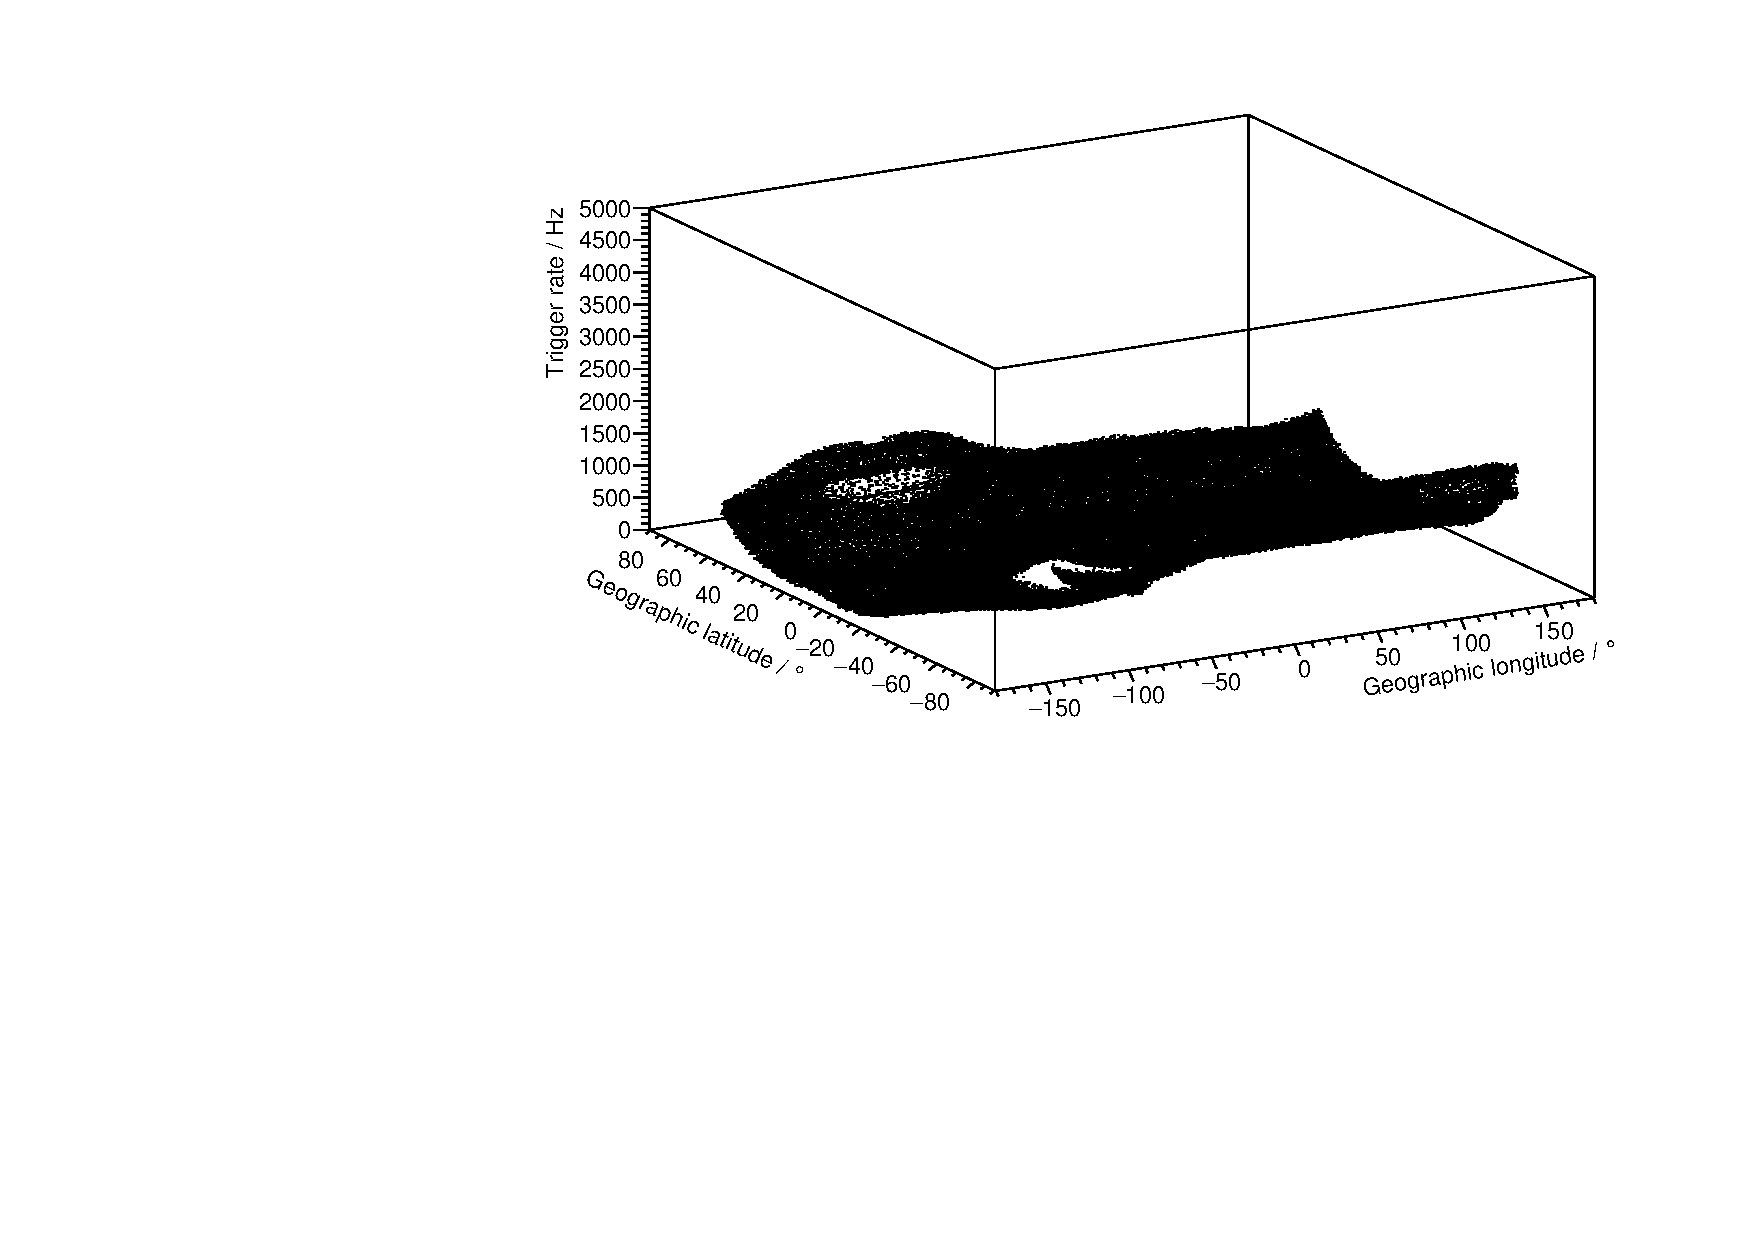
\includegraphics[width=0.47\textwidth, height=0.29\textheight]{Figures/chapter4/MeasuringTime/TriggerRateVsPosition.pdf}
%	\label{TriggerRateVsPosition}
%    }
%    \caption[]{a). Live time fraction vs. ISS position. b). Trigger rate vs. ISS position}
%\end{figure}
%\end{comment}
% End Comment out

\begin{figure}[htpb]
\centering
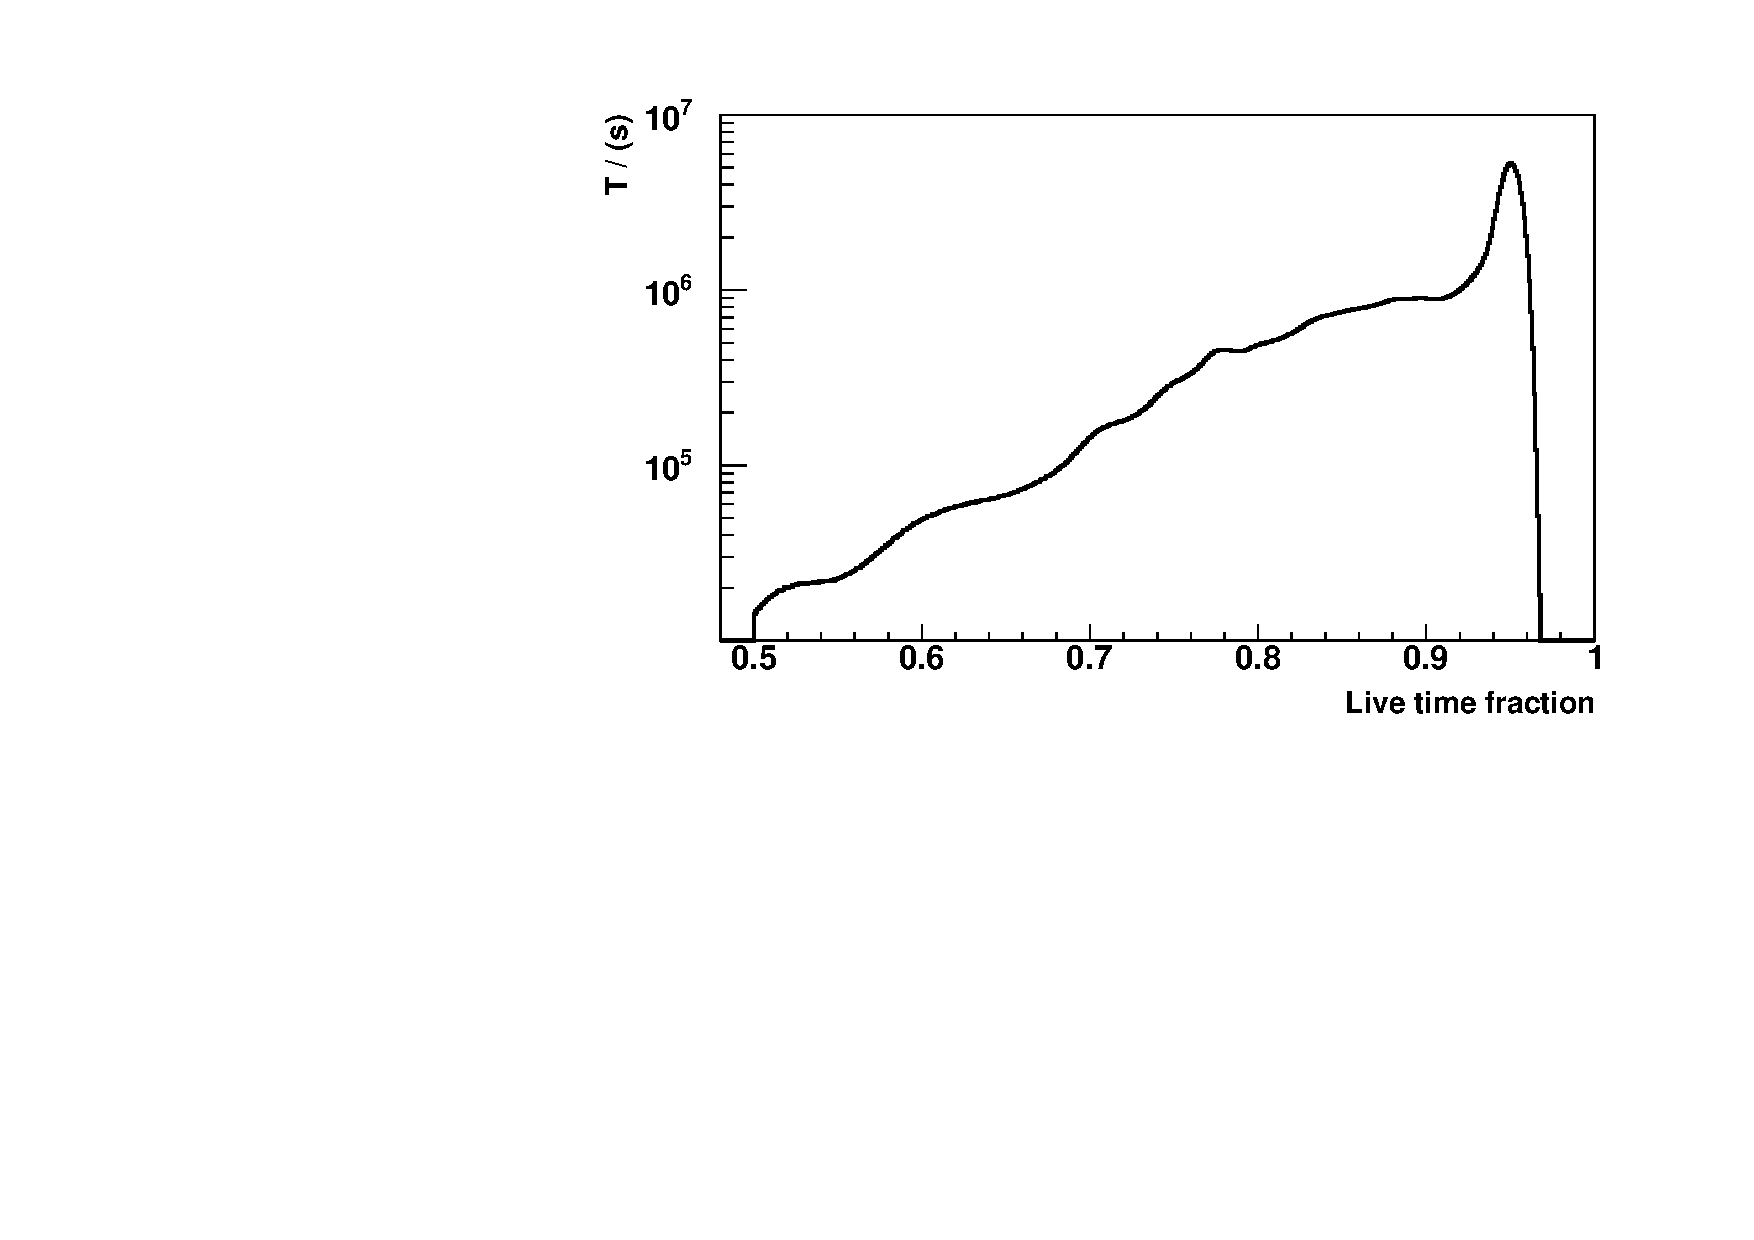
\includegraphics[width=1.0\textwidth]{Figures/chapter4/MeasuringTime/MeasuringTimeVsLiveTime.pdf}
\caption[Measuring time as a function of the live time fraction.]{Measuring time as a function of the live time fraction. For most of the measuring time, the live time fraction is above 0.9.}
\label{MeasuringTimeVsLiveTime}
\end{figure}
 
% Start Comment out
%\begin{comment} 
%\begin{figure}[p]
%\centering
%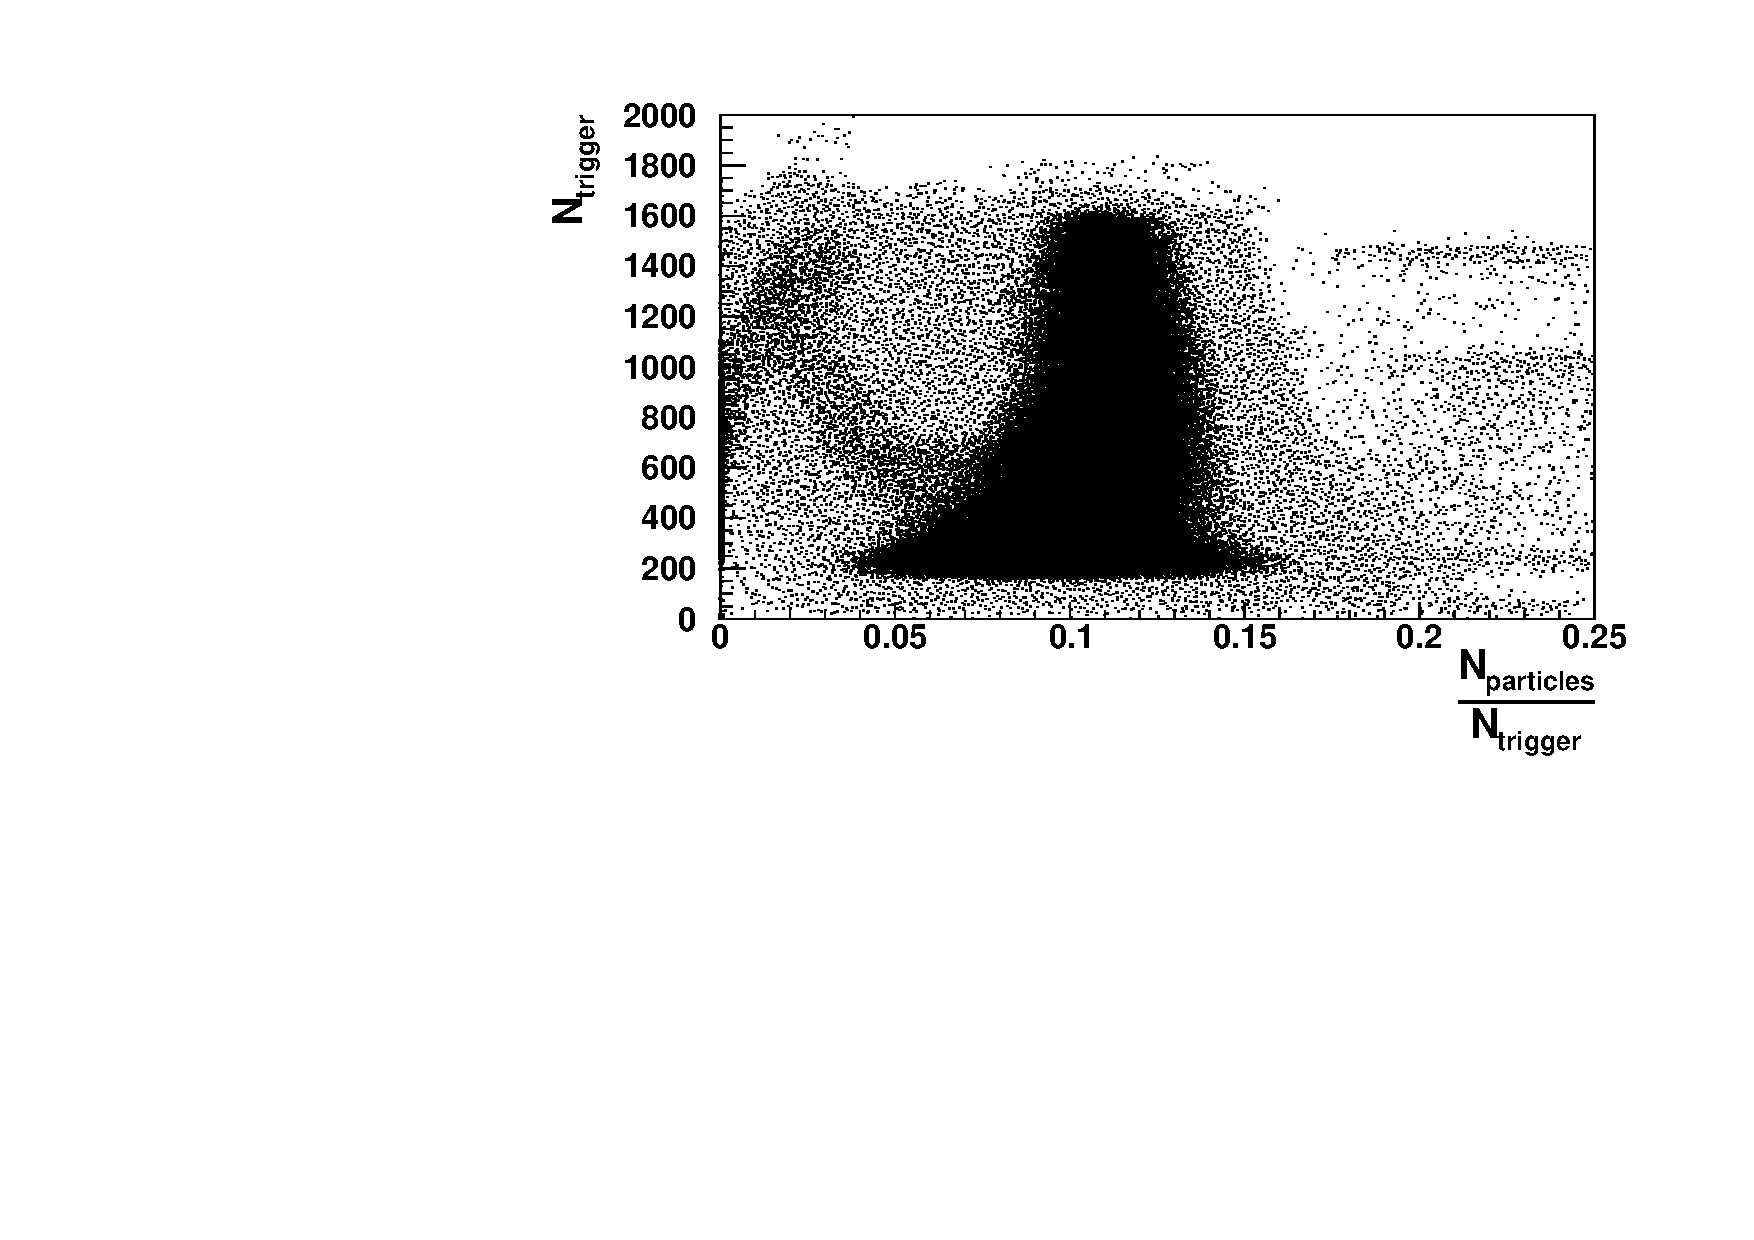
\includegraphics[width=1.0\textwidth, height=0.37\textheight]{Figures/chapter4/MeasuringTime/ParticlesVsTriggers.pdf}
%\caption[]{Triggers as a function of particles over trigger ratio.} 
%\label{ParticlesVsTriggers}
%\end{figure}
%\end{comment}
% End Comment out

%% Earth magnetic field 
\begin{figure}[htb]
\centering
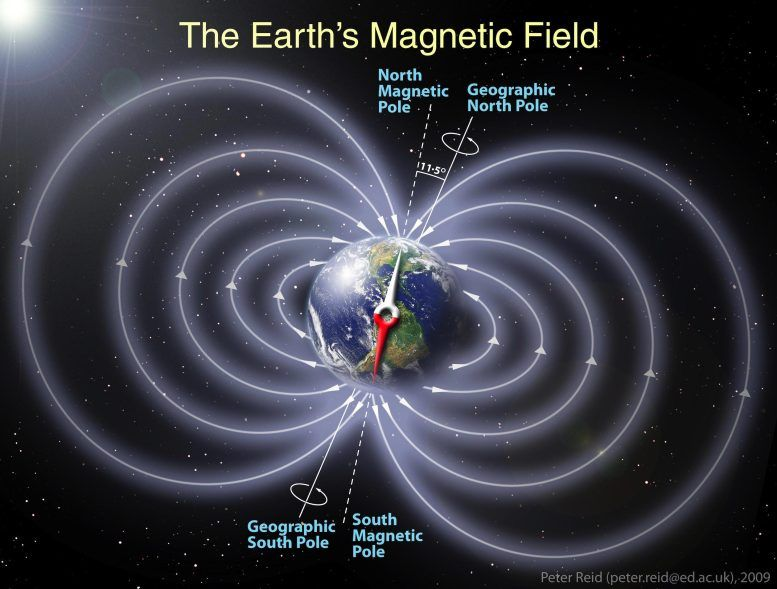
\includegraphics[width=0.9\textwidth, height=0.37\textheight]{Figures/chapter4/MeasuringTime/Earths-Magnetic-Field-Schematic-Illustration.jpg}
\caption[Illustration of the Earth’s magnetic field.]{Illustration of the Earth’s magnetic field. The angle between the Earth’s magnetic field axis and the Earth’s rotational axis is $11.5^{\circ}$. Credit: Peter Reid, The University of Edinburgh}
\label{EarthMagneticField}
\end{figure}

Due to the Earth's magnetic field, a charged particle can be deflected before it reaches the detectors at low earth orbit, where the AMS-02 is located. The deflection power depends on the particle's rigidity and the particle's relative orientation to the magnetic field lines. \par

The Earth’s magnetic field axis is tilted at an angle of $11.5^{\circ}$ with respect to the Earth’s rotational axis, as illustrated in figure \ref{EarthMagneticField}. Therefore, the lowest rigidity threshold to penetrate the Earth's magnetic field should be a function of the Earth's location. The lowest rigidity threshold is called $\textit{rigidity cutoff}$. \par    

To get rid of these events which are deflected by the Earth's magnetic field, the following requirement is applied: 
\begin{equation}
R_\mathrm{low} > R_{c} \times f 
\end{equation}

where $f$ is the safety factor, which is set to be 1.2 in this analysis, $R_{c}$ is the cutoff rigidity,  and $R_\mathrm{low}$ is the lower edge of rigidity bin, which in the measured rigidity is classified.  \par


%% Cutoff and Measuring time
% Størmer Cutoff
For the rigidity cutoff, there are two kinds of cutoffs used in the AMS-02 collaboration: Størmer cutoff and International Geomagnetic Reference Field (IGRF) cutoff. The Størmer cutoff is only valid for the approximation of a pure dipole field. Since the geomagnetic field deviates from a pure dipole field, the IGRF cutoff takes deformations in the geomagnetic field into account and therefore more accurate. Both of the two cutoffs will be discussed in this section.\par

For the Størmer rigidity cutoff, the equation \ref{StormerCutoffCalculation} gives the formula to calculate the cutoff $R_{c}$ \cite{StormerCutOffCalculation}:  

\begin{equation}
\label{StormerCutoffCalculation}
R_{c} = \frac{M{\rm{cos}}^4\lambda}{r^2(1+\sqrt{1- \rm{sin} \epsilon \cdot \rm{sin} \delta \cdot \rm{cos}^3 \lambda } )^2}
\end{equation}

where $M$ is the geomagnetic dipole moment with a typical value of 58 \cite{StormerCutOffEquation}, $\lambda$ is the magnetic latitude, $r$ is the altitude distance from the dipole center, $\epsilon$ and $\delta$ are the zenith and azimuthal angles of the particle, respectively.

%(High: RigidityAboveIGRFCutoff(35PN|1.2).  Low:  RigidityAboveGeomagneticCutoff(25PN|1.2) )
With the cuts and selection introduced in Section \ref{DataSelectionSection}, the calculated Størmer rigidity cutoff for events with zenith angle up to 25$^{\circ}$ as a function of ISS position is given in figure \ref{StormerCutOffRigidity}. 

% Størmer Measuring Time 
The total measuring time can be obtained by integrating the live time fraction in every second of the whole data-taking period. 

\begin{figure}[hptb]
\centering
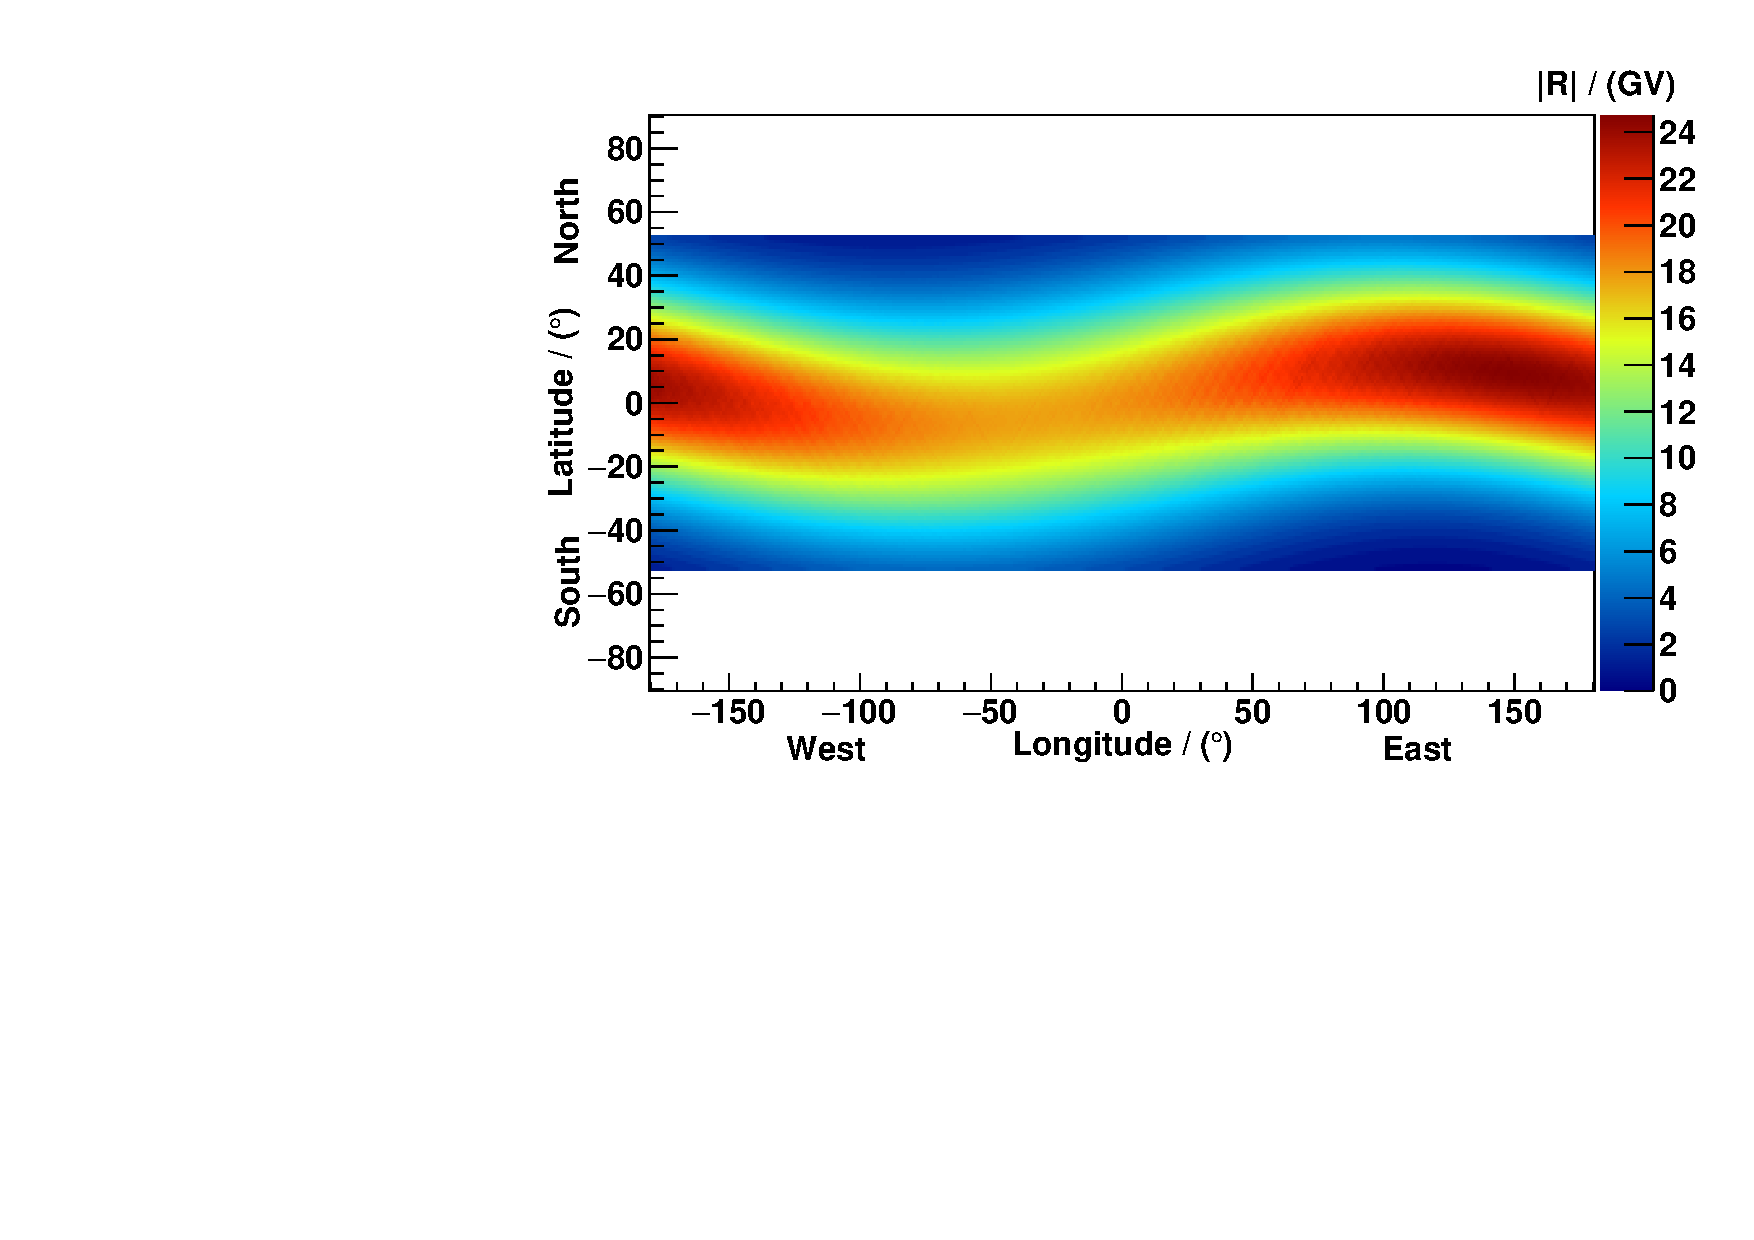
\includegraphics[width=1.0\textwidth, height=0.41\textheight]{Figures/chapter4/MeasuringTime/CutOffRigidityVsISSPosition.pdf}
\caption[The Størmer rigidity cutoff as a function of the ISS Position.]{The Størmer rigidity cutoff used in this analysis as a function of the ISS Position. The maximum value of the cutoff is less than 26 GV.}
\label{StormerCutOffRigidity}
\end{figure}


\begin{figure}[hptb]
\centering
\includegraphics[width=1.0\textwidth, height=0.41\textheight]{Figures/chapter4/MeasuringTime/Measuringtime.pdf}
\caption[The measuring time from the Størmer geomagnetic cutoff.]{The measuring time obtained from the Størmer geomagnetic cutoff. After the quality cuts and live time fraction, the resulting total measuring time is around 2488 days.}
\label{Measuringtime}
\end{figure}

\begin{figure}[htpb]
\centering
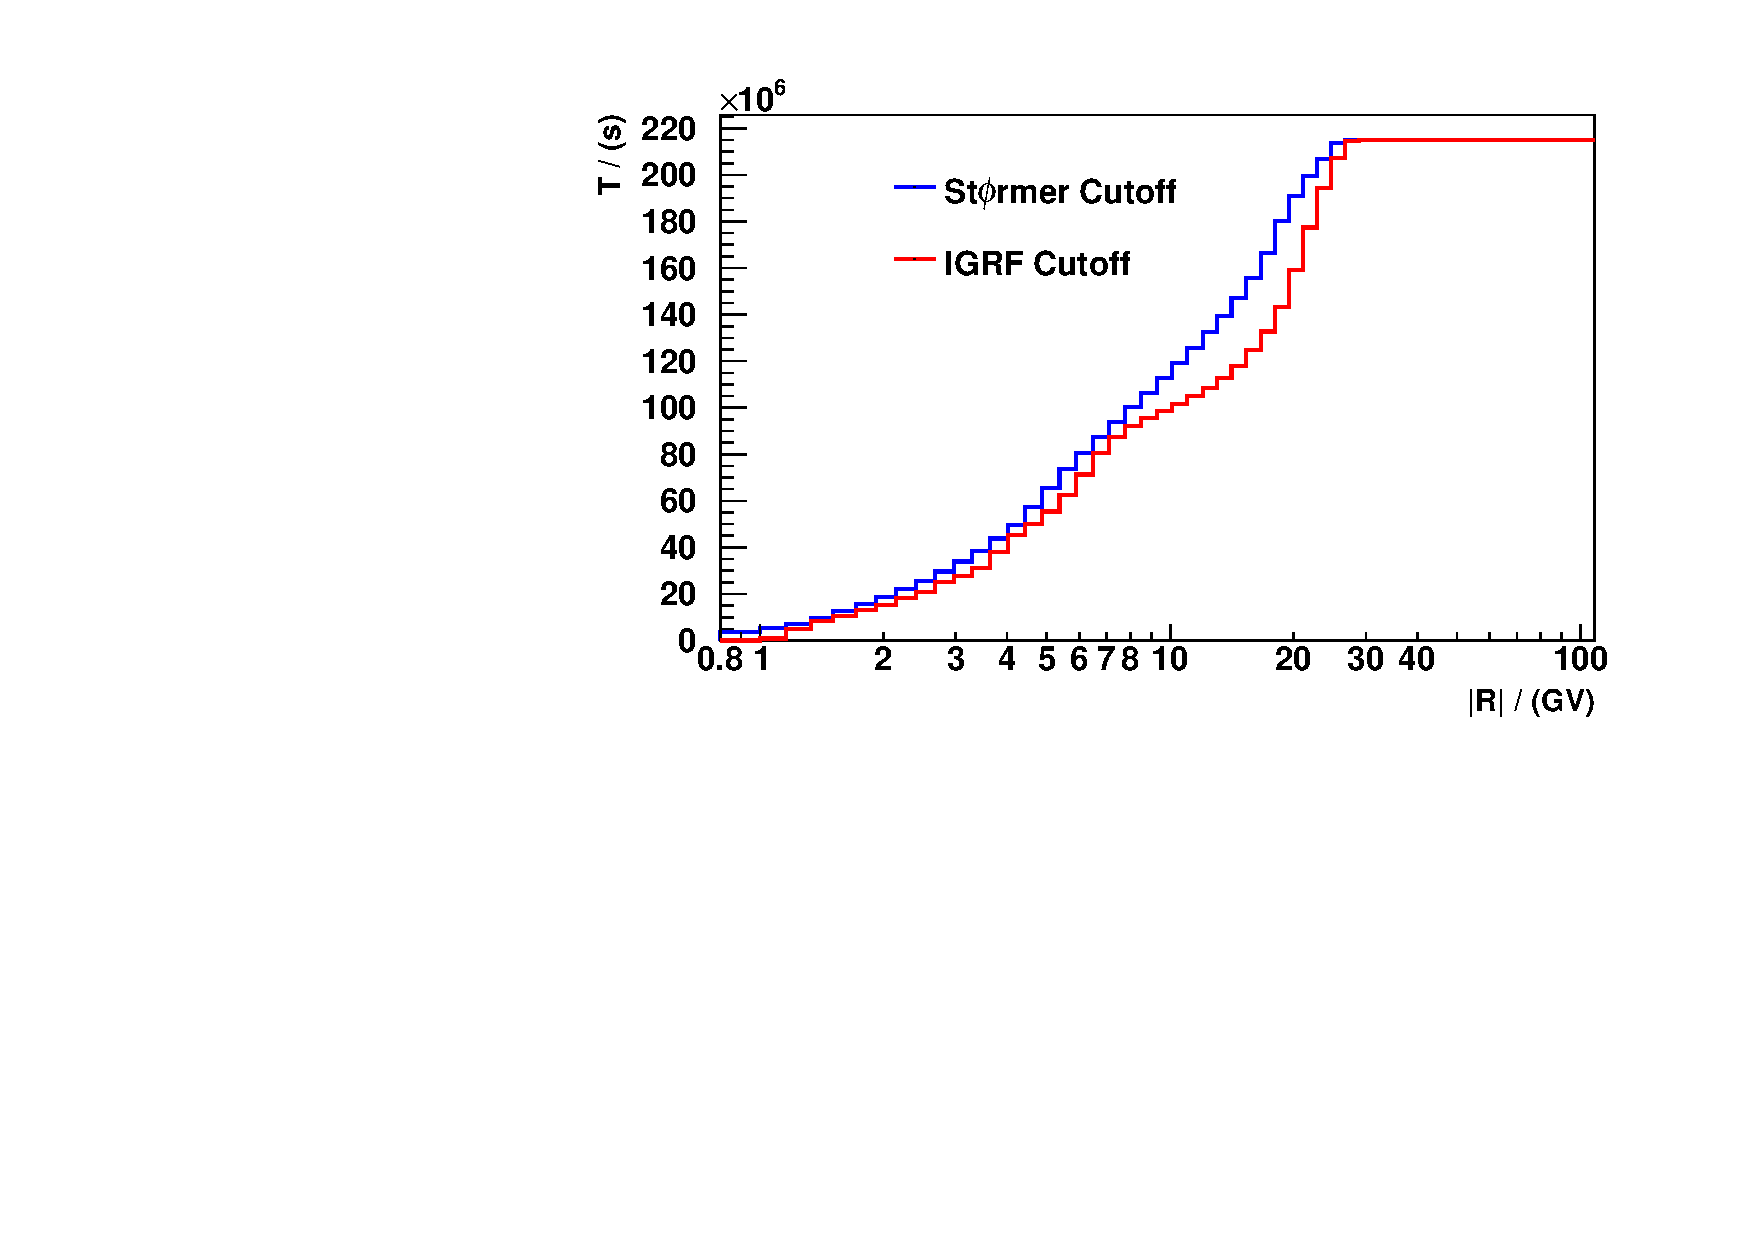
\includegraphics[width=1.0\textwidth, height=0.41\textheight]{Figures/chapter4/MeasuringTime/IGRFvsStomer.pdf}
\caption[The measuring time comparison between the Størmer and IGRF cutoffs.]{The measuring time comparison between the Størmer and IGRF cutoffs. The IGRF cutoff leads to lower measuring time.}
\label{IGRFvsStomer}
\end{figure}

After the preselection cuts introduced in Section \ref{DataSelectionSection} which ensure good operation quality of the sub-detectors, the resulting measuring time as a function of rigidity used in this analysis is shown in figure \ref{Measuringtime}. The integrated data-taking time from 20. May 2011 to 03. May 2021 is 3636 days. Due to the ISS position, detector operations like TRD gas refills and the time spent inside the SAA, the actual measuring time is around 68\% of the total data taking time. This leads to a measuring time of 2488 days above the geomagnetic cutoff.  %actual number for 2488days is: 2.1497933e+08 s

% IGRF cutoff
Another method used by the AMS-02 collaboration to calculate the rigidity cutoff is the IGRF method. To calculate the track of particle which penetrates the magnetic field, a solution is to consider the backtracing particles. With a given position and a specified rigidity, the back-trajectory of a charged particle can be traced by numerical integration through a mathematical model of the geomagnetic field, IGRF model, until the particle either reaches the interplanetary magnetic field, or intersects the atmosphere. In this way, the threshold of rigidity is the cutoff rigidity for this position.  \par
%If all the backtracing particles from a certain position and rigidity are primary particles, namely from outer space, the rigidity is the cutoff rigidity for this position. 
%The magnetic field model should be determined first in this numerical calculation of backtracing particles. One model option is the International Geomagnetic Reference Field (IGRF) model. Therefore, the name for calculating the rigidity cutoff is called IGRF method. \par
% the path of a charge particle with a specified rigidity is traced by numerical integration thrrough a mathematical model of the geomagnetic field until tthe particle either reaches the interplanetary magnetic field (allowed orbit), intersects the solid earth (forbiden orbit) or becomes 'quasi-trapped'.

% Comparison: IGRF & Stormer


Figure \ref{IGRFvsStomer} shows the comparison between the measuring time achieved from the IGRF method and the Størmer cutoff method. As shown in the figure, compared to the IGRF method, using the Størmer cutoff leads to higher statistics in the low rigidity range. This is important for the time-dependent analysis since the statistics in the fine time bin are limited. Also, using the IGRF method leads to almost zero measuring time in the first one to two rigidity bins (less than 1.16 GV). Therefore, the data could only be analyzed in the higher rigidity bins. So in this analysis, the Størmer cutoff is used to determine the measuring time though it is based on the approximation of the dipole field.

% Time-dependent Measuring Time

\begin{figure}[hptb]
\centering
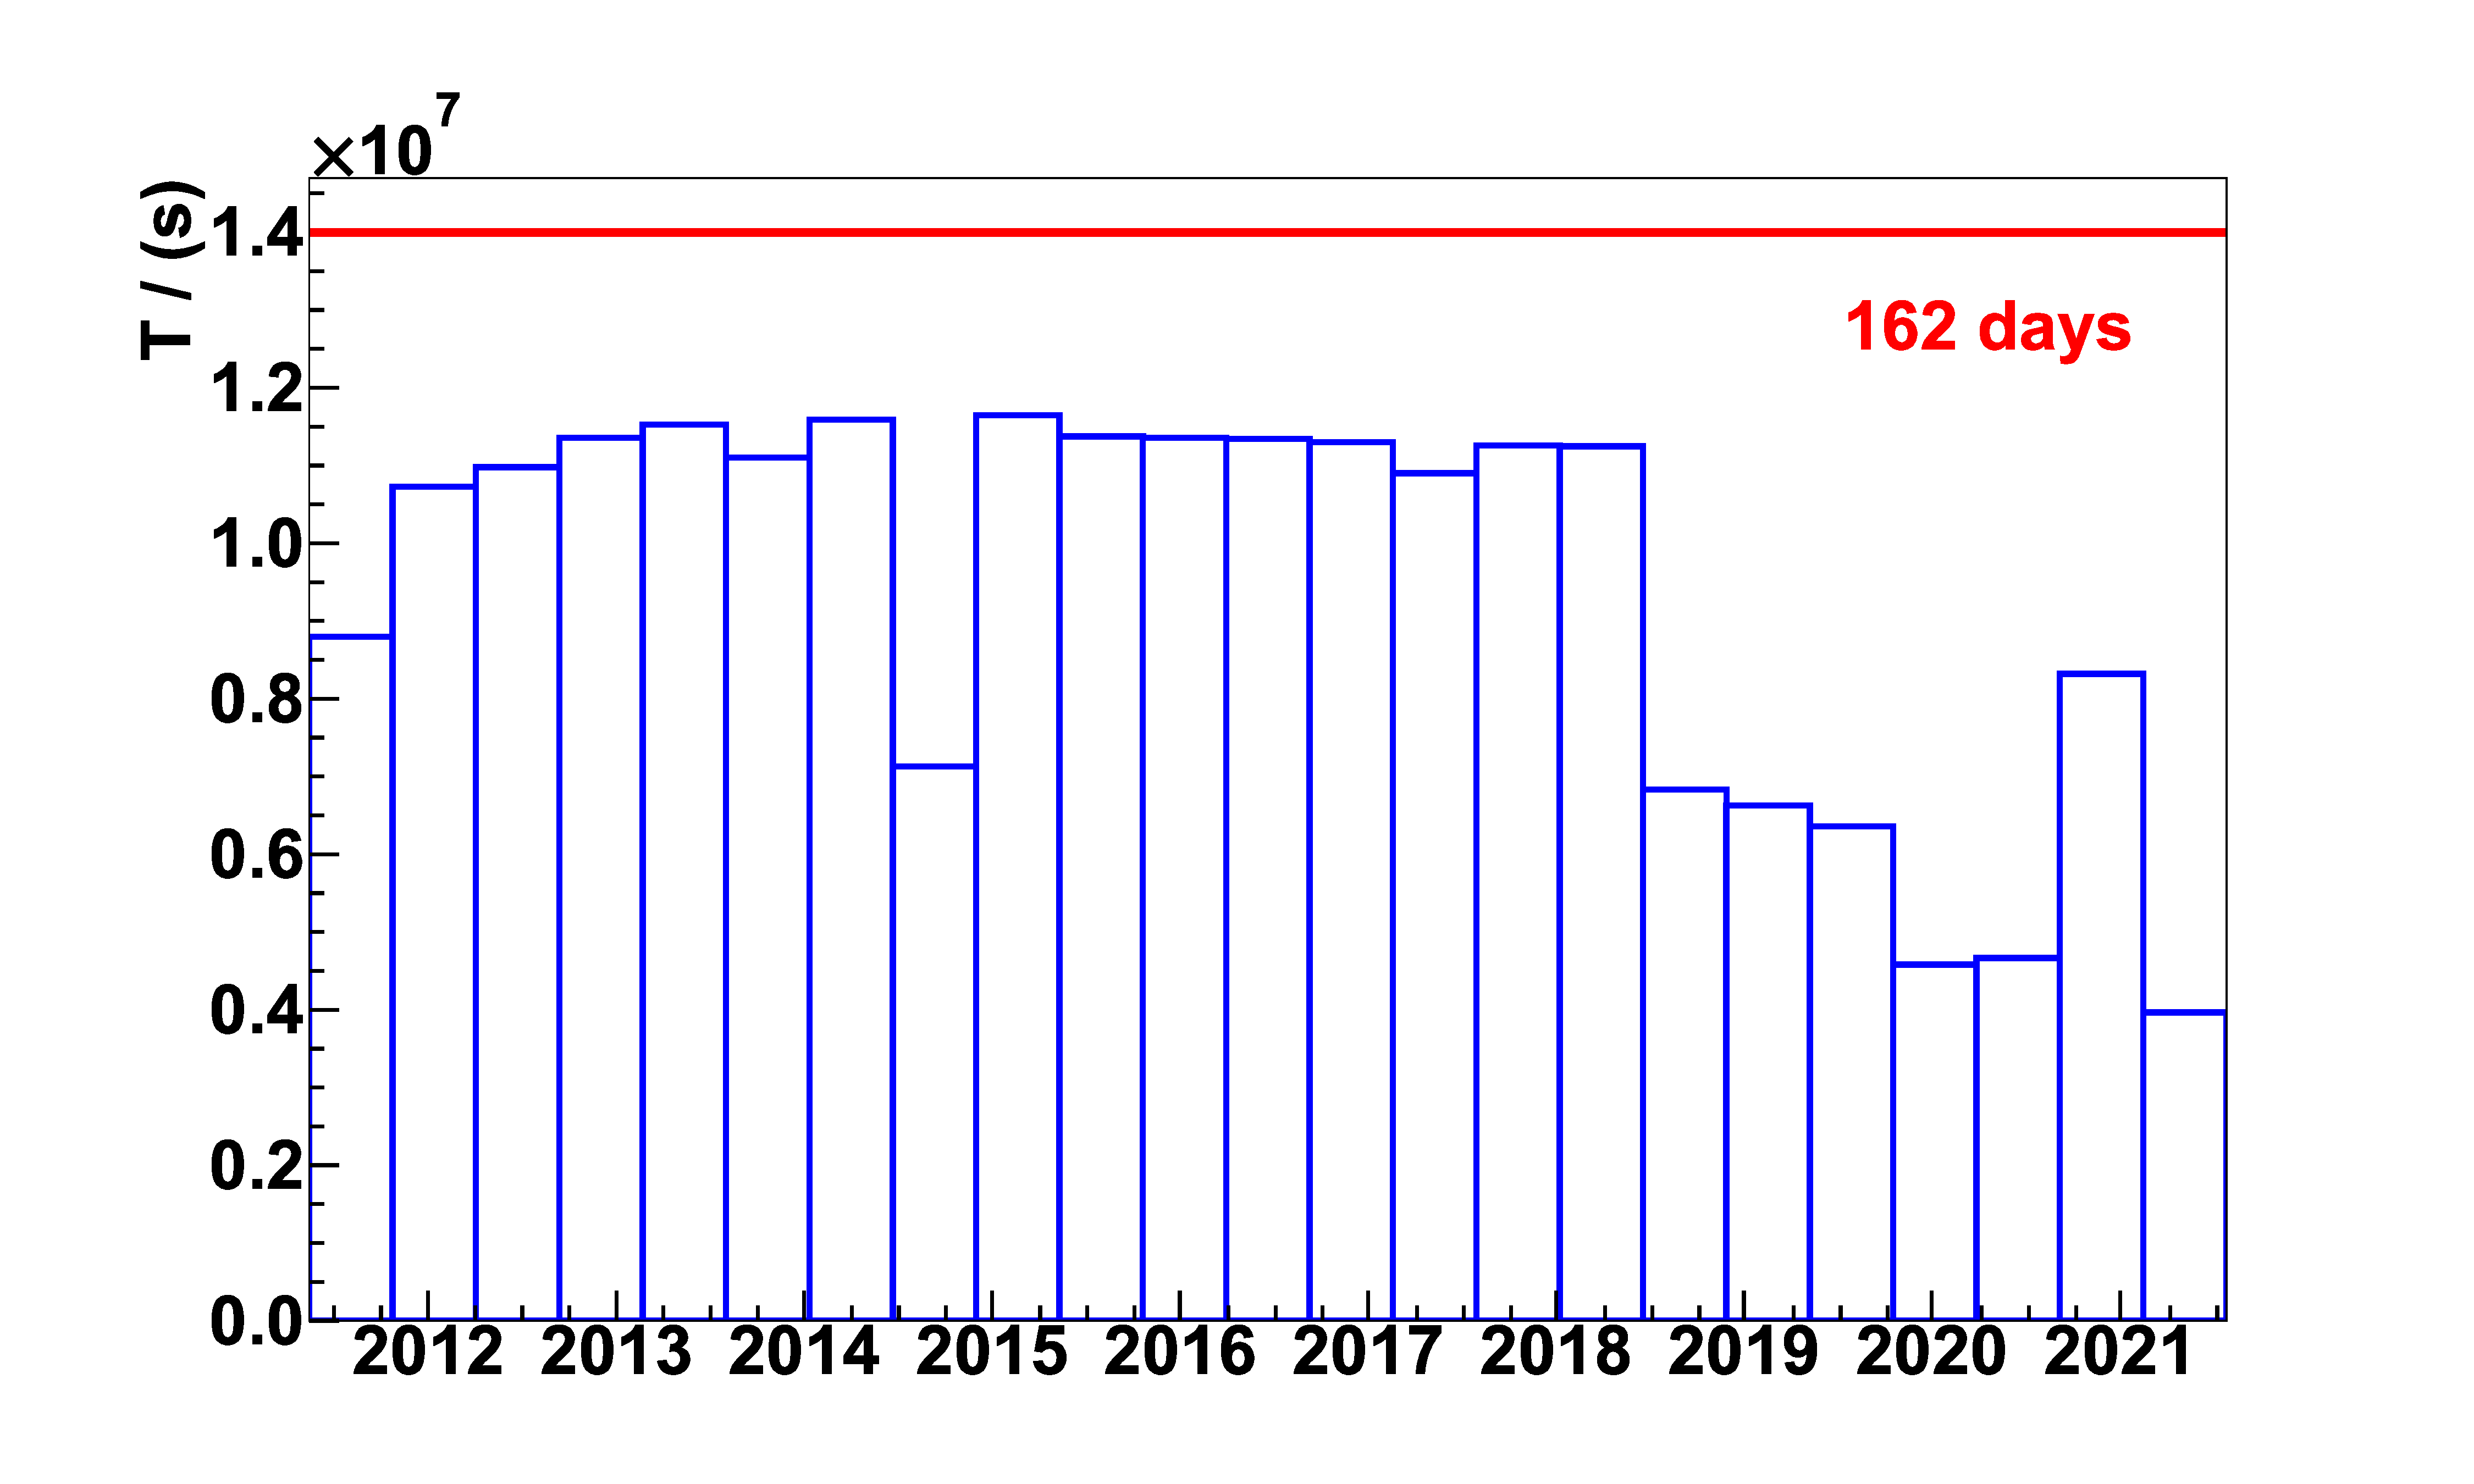
\includegraphics[width=1.0\textwidth, height=0.4\textheight]{Figures/chapter4/MeasuringTime/TimeDependent/TimeDependentMeasuringTime.pdf}
\caption[The measuring time in each six Bartels Rotations time bin.]{The measuring time in each six Bartels Rotations time bin. After the middle of 2018, the measuring time in each time bin decreased due to frequent changes of the pump running status. The red line indicates the exact six Bartels Rotations (162 days).}
\label{TimeDependentMeasuringTime}
\end{figure}    

For the time-dependent analysis, the collected ISS data is divided into every six Bartels Rotations time bin. In each time bin, the total measuring time depends on the detector operation in these individual six Bartels Rotations. In figure \ref{TimeDependentMeasuringTime}, the measuring time in the 23 six Bartels Rotations time bins is shown.












